\chapter{Oscilaciones}
\refstepcounter{subsection}
Usualmente estudiamos oscilaciones sinusoidales, pero cualquier oscilación periórida en torno a una posición de equilibrio también es sujeto de estudio. Sin embargo, las ondas sinusoidales juegan un papel especial.

Si tenemos un potencial $U(\mathbf{x})$ con un mínimo local en $\mathbf{x}_0$, podemos expandirlo por taylor en torno a ese mínimo, tal que
\begin{equation} \label{6.1.1}
    U(\mathbf{x}) = U(\mathbf{x}_0) + \nabla U (\mathbf{x}_0) \cdot (\mathbf{x}-\mathbf{x}_0) + \frac{1}{2}(\mathbf{x}-\mathbf{x}_0)^T \mathbb{H}_U (\mathbf{x}_0)(\mathbf{x}-\mathbf{x}_0) + O((\mathbf{x}-\mathbf{x}_0)^3)
\end{equation}\refstepcounter{subsection}
Donde $\nabla U$ es el gradiente del potencial, evaluado en el mínimo, por lo tanto se anula, y $\mathbb{H}_U$ es la hessiana evaluada en $\mathbf{x}_0$.

Si ahora despreciamos los términos de orden cúbico y superiores, y hacemos el gradiente de (8.0.1), el primer término constante se anula, y entonces tenemos que 
\[
    \frac{\partial U}{\partial x_i} = \frac{1}{2}\frac{\partial}{\partial x_i} \sum_{jk} H_{jk} (x_j-x_{0_j})(x_k-x_{0_k}) = \frac{1}{2}\sum_{jk} H_{jk} \delta_{ij} (x_k-x_{0_k}) + \frac{1}{2}\sum_{jk} H_{jk} \delta_{ik} (x_j-x_{0_j})
\] \vspace{-15pt}
\begin{equation} \label{6.1.1}
    = \sum_{jk} H_{jk} \delta_{ij} (x_k-x_{0_k}) = \sum_{k} H_{ik} (x_k-x_{0_k}) \iff \nabla U = \mathbb{H}_U (\mathbf{x}_0)(\mathbf{x}-\mathbf{x}_0)
\end{equation}\refstepcounter{subsection}
Se puede demostrar que $\mathbf{A} = \mathbb{H}_U (\mathbf{x}_0)$ es definida positiva al tratarse de un mínimo. En el caso unidimensional esto se reduce a 
\begin{equation} \label{6.1.1}
    \frac{dU}{dx} = k (x-x_0) \ \ \ \ \ \ k = \frac{d^2 U}{dx^2}(x_0) > 0
\end{equation}\refstepcounter{subsection}
Usando la 2LN llegamos al oscilador harmónico cuyas soluciones son oscilaciones sinusoidales
\begin{equation} \label{6.1.1}
    m\ddot{x} = - k(x-x_0) \implies x = x_0 + A\cos(\omega_0 t - \delta)\ \ \ \ \ \omega_0^2 = \frac{k}{m}
\end{equation}\refstepcounter{subsection}
\vspace{-25pt}
\section{Oscilaciones sinusoidales}
\refstepcounter{subsection}
La ecuación (8.0.4) puede ser escrita de las siguientes formas equivalente
\begin{equation} \label{6.1.1}
    x = x_0 + C_1e^{i\omega_0t}+ C_2e^{-i\omega_0t} = x_0 + C_1'\cos\omega_0 t + C_2'\sin \omega_0 t
\end{equation}\refstepcounter{subsection}
\vspace{-25pt}
\begin{equation} \label{6.1.1}
    x = x_0 + A\left(\cos\delta\cos\omega_0 t + \sin\delta\sin \omega_0 t\right) \ \ \ \ \ A^2 = C_1'^2+C_2'^2 \ \ \ \ \ \sin\delta = \frac{C_2'}{A} \ \ \ \ \cos\delta = \frac{C_1'}{A}
\end{equation}\refstepcounter{subsection}
\vspace{-15pt}
\begin{equation} \label{6.1.1}
    x =  x_0 + \mathfrak{Re}\{C e^{i\omega_0t}\} \ \ \ \ \ \ C = A e^{-\delta}
\end{equation}\refstepcounter{subsection}
\subsection{Energía}
La energía de un oscilador harmónico general es 
\begin{equation} \label{6.1.1}
    U = \frac{1}{2}(\mathbf{x}-\mathbf{x}_0)^T \mathbb{H} (\mathbf{x}-\mathbf{x}_0)
\end{equation}\refstepcounter{subsection}
y para el caso unidimensional se reduce a 
\begin{equation} \label{6.1.1}
    U = \frac{1}{2}k(x-x_0)^2 = \frac{1}{2}kA^2 \cos^2(\omega_0t-\delta)
\end{equation}\refstepcounter{subsection}
por otro lado, tenemos que la energía cinética para el caso unidimensional es 
\begin{equation} \label{6.1.1}
    T = \frac{1}{2}m(x-x_0)^2 = \frac{1}{2}\underbrace{m\omega_0^2}_k A^2 \sin^2(\omega_0t-\delta)
\end{equation}\refstepcounter{subsection}
Y entonces, en ausencia de fuerzas externas, la energía es
\begin{equation} \label{6.1.1}
    E = T+U = \frac{1}{2} k A^2
\end{equation}\refstepcounter{subsection}
\vspace{-25pt}
\subsection{Oscilaciones en más dimensiones}
Para cualquier número de dimensiones, tenemos que
\begin{equation} \label{6.1.1}
    m\ddot{\mathbf{x}} = -\nabla U = -\mathbb{H} (\mathbf{x}-\mathbf{x}_0) 
\end{equation}\refstepcounter{subsection}
La matriz $\mathbb{H}$ es real y simétrica, y por tanto hermítica, y por lo tanto existe una base en la que diagonaliza, tal que si $\mathbf{x}' = \mathbf{x}-\mathbf{x}_0$, entonces
\begin{equation} \label{6.1.1}
    m\ddot{\mathbf{x}}' = -\mathbb{H} \mathbf{x}' = \left(\begin{matrix}
        -k_1 x_1' \\ -k_2 x_2' \\ -k_3 x_3'
    \end{matrix}\right)
\end{equation}\refstepcounter{subsection}
Vamos a centrarnos en dos dimensiones, en el primer caso, si los autovalores $k_1$ y $k_2$ son iguales a $k$, lo que se denomina isótropo, tenemos que
\begin{equation} \label{6.1.1}
    \left\{\begin{matrix}
        x(t) = A_x \cos(\omega_0t - \delta_x) \\
        y(t) = A_y \cos(\omega_0t - \delta_y) 
    \end{matrix}\right. \ \ \ \ \ \omega_0^2 = \frac{k}{m}
\end{equation}\refstepcounter{subsection}
y definiendo $t' = t-t0$ tal que $t_0 = \delta_x/\omega_0$, definimos $\delta = \delta_y-\delta_x$, entonces tenemos
\begin{equation} \label{6.1.1}
    \left\{\begin{matrix}
        x(t) = A_x \cos(\omega_0t) \phantom{--}\\
        y(t) = A_y \cos(\omega_0t - \delta) 
    \end{matrix}\right.
\end{equation}\refstepcounter{subsection}
Lo que corresponde a la ecuación de una elipse, que en general puede estar rotada.

Si es anisótropo, es decir, los autovalores no coinciden, solo realizará trayectorias periódicas si 
\begin{equation} \label{6.1.1}
    \frac{\omega_0_x}{\omega_0_y} = \frac{p}{q} \rightarrow \tau = \frac{2\pi p}{\omega_0_x} = \frac{2\pi q}{\omega_0_y} \implies \left\{\begin{matrix}
        x(t+\tau) = A_x \cos(\omega_0_xt + \omega_0_x \tau -\delta_x) = x(t) \\
        y(t+\tau) = A_y \cos(\omega_0_yt +\omega_0_y \tau- \delta_y) = y(t)
    \end{matrix}\right.
\end{equation}\refstepcounter{subsection}
En función de ese cociente, las trayectorias trazadas se llaman curvas de Lissajous.
\section{Oscilaciones amortigudas}
Si añadimos una fuerza que se opone linealmente a la velocidad de la forma $-b \dot{x}$ (para una dimensión), obtenemos la siguiente ecuación diferencial.
\begin{equation} \label{6.1.1}
    \ddot{x} + 2\beta\dot{x} + \omega_0^2 x = 0 \ \ \ \ \ 2\beta = \frac{b}{m} \ \ \ \ \ \omega_0^2 = \frac{k}{m}
\end{equation}\refstepcounter{subsection}
La solución va a ser de la forma $e^{\alpha t}$, de tal forma que los valores de alpha vienen dados por la ecuación auxiliar
\begin{equation} \label{6.1.1}
    \alpha^2 + 2\beta\alpha + \omega_0^2= 0 \implies \alpha = -\beta \pm \sqrt{\beta^2-\omega_0^2}
\end{equation}\refstepcounter{subsection}
De esta forma, tendremos tres soluciones distintas en función del valor de $\beta$
\subsection{Subamortiguamiento}
Para el caso en el que $\beta < \omega_0$, tenemos que $\alpha = -\beta \pm i \sqrt{\omega_0^2-\beta^2} = -\beta \pm i \omega'$, entonces las soluciones son de la forma (8.0.4) con un prefactor, tal que
\begin{equation} \label{6.1.1}
    x(t) = e^{-\beta t}A\cos(\omega't-\delta)
\end{equation}\refstepcounter{subsection}
Es decir, tenemos oscilaciones sinusoidales que se van extinguiendo conforme pasa el tiempo, es decir, su amplitud disminuye exponencialmente y el factor que determina esa desaparición, llamado parámetro de extinción, es $\beta$.
\subsection{Sobreamortiguamiento}
Para el caso en el que $\beta > \omega_0$, tenemos que $\alpha = -\beta \pm \sqrt{\beta^2-\omega_0^2}$ reales ambos, tal que $0<a_1 =\beta - \sqrt{\beta^2-\omega_0^2} < a_2 = -\beta + \sqrt{\beta^2-\omega_0^2}$, de tal forma que las soluciones son de la forma
\begin{equation} \label{6.1.1}
    x(t) = C_1 e^{-a_1t}+ C_2 e^{-a_2t}
\end{equation}\refstepcounter{subsection}
De tal forma que como $a_2 > a_1$ el primer término es el que primará a tiempos largos y por lo tanto el parámetro de extinción será $a_1$.

En este caso ya no tenemos oscilaciones sinusoidales, y en función de las condiciones iniciales, como por ejemplo una velocidad inicial en la posición de equilibrio, tendremos que hace solo una oscilación, es decir llega a una distancia máxima y a partir de ahí vuelve a la posición de equilibrio sin oscilar más.
\subsection{Amortiguamiento crítico}
En el caso en el que $\beta = \omega_0$ tendremos que $\alpha = -\beta$, por lo que como segunda solución linealmente independiente propondremos $te^{\alpha t}$, entonces las ssoluciones nos quedan
\begin{equation} \label{6.1.1}
    x(t) = C_1 e^{-\beta t}(1+C_2t)
\end{equation}\refstepcounter{subsection}
Y de nuevo $\beta$ es el parámetro de extinción.

\begin{center}
    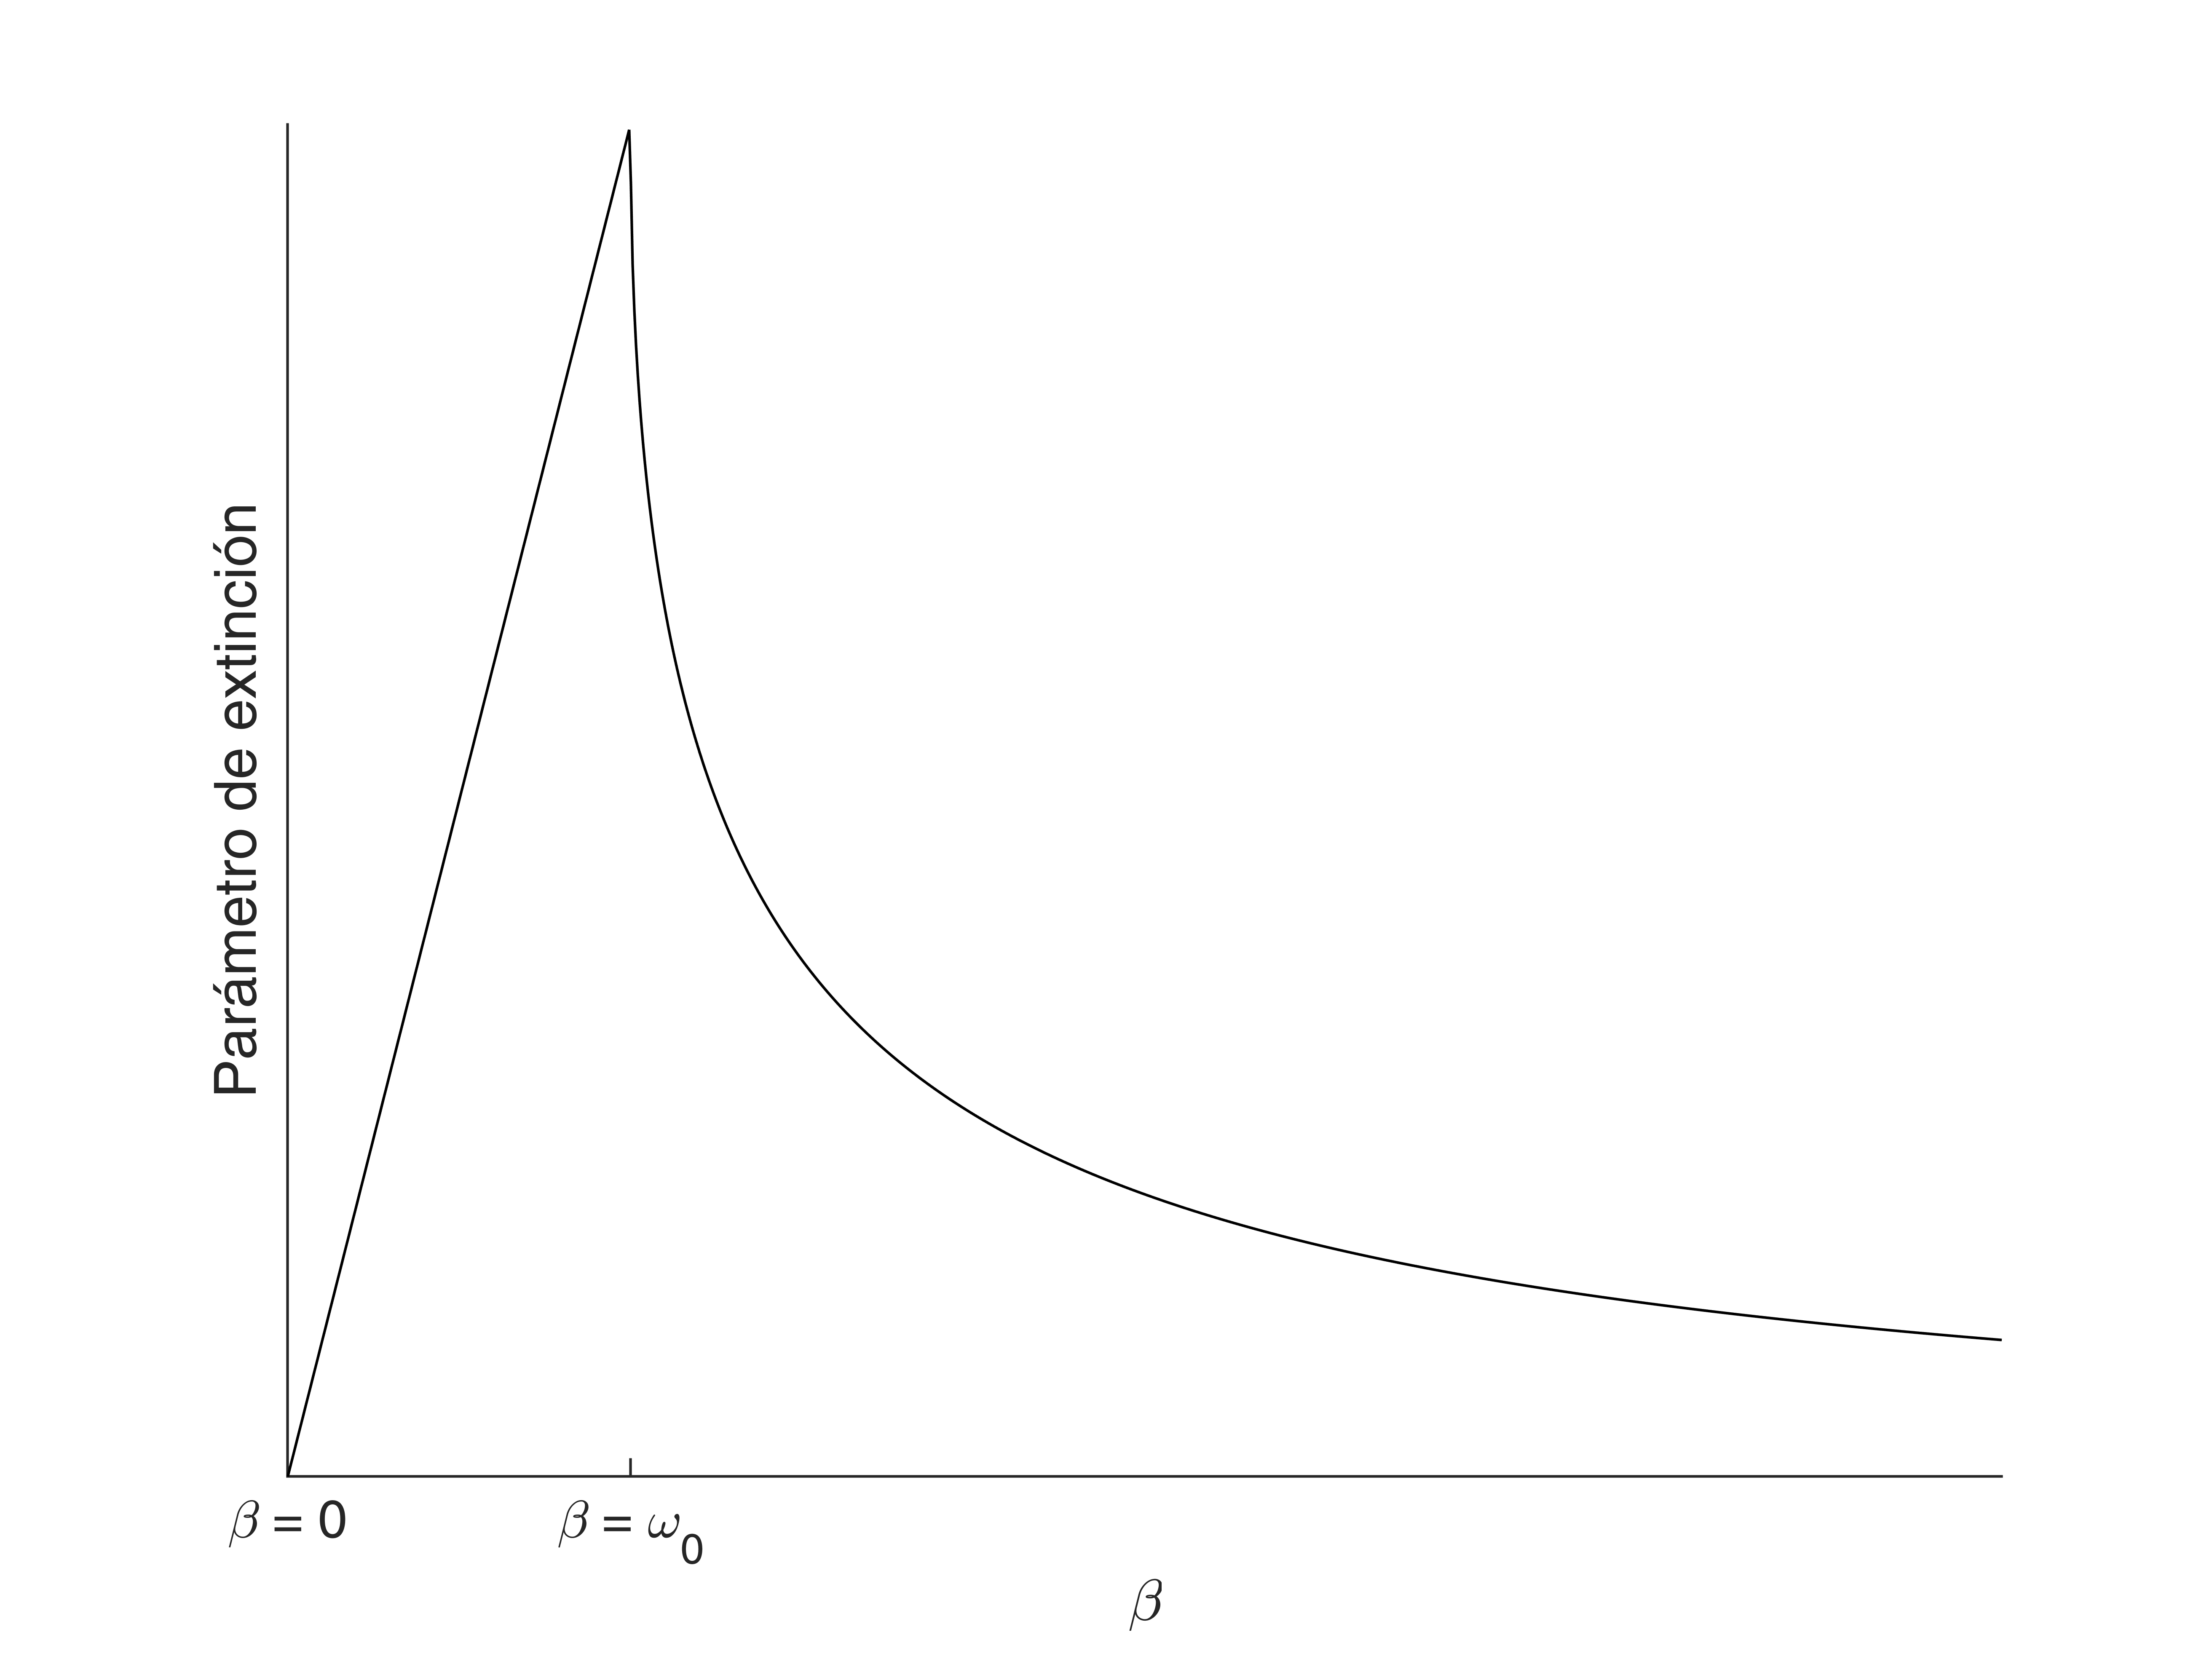
\includegraphics{extin.png}    
\end{center}

Si representamos el parámetro de extinción en función de $\beta$ utilizando las expresiones que hemos ido hallando, observamos que la mayor amortiguación ocurre cuando $\beta = \omega$, por eso se llama amortiguamiento crítico.

A mayores $\beta$, hay menos posibilidad de amortiguamiento por que el sistema casi no oscila y por lo tanto la velocidad va a ser pequeña.

\section{Oscilaciones forzadas}